% =====================================================================
% Mass-Aware Routing — preview document for sections completed so far.
% Compile: pdflatex paper_main.tex (twice for refs)
% =====================================================================
\documentclass[11pt]{article}
\usepackage[a4paper,margin=2cm]{geometry}
\usepackage[ruled,vlined]{algorithm2e}
\usepackage{amsmath, amssymb}
\usepackage{graphicx}
\usepackage{cite}
\usepackage{booktabs}
\usepackage{xcolor}
\usepackage{hyperref}
\hypersetup{colorlinks=true, linkcolor=blue!50!black, citecolor=blue!50!black}

\SetKwInOut{Input}{Input}
\SetKwInOut{Output}{Output}
\SetKwProg{Fn}{Function}{:}{}

% Allow \begin{keyword} from Elsevier abstract block to work in plain article
\providecommand{\sep}{,}\newenvironment{keyword}{\paragraph{Keywords:}\itshape}{\par}

\title{EMMET: Effective-Mass Memory Edge Transport \\ \large Per-Packet State for Stateful Adaptive Routing}
\author{Carlos L\'opez}
\date{Draft \today}

\begin{document}
\maketitle

% =====================================================================
% Abstract for EMMET-Newt paper (v2.0+).
% Target venue: IEEE TNSM, Computer Networks (Elsevier).
% Length: 200-280 words.
% Tone: framework contribution, mechanistic vocabulary, no hype.
% =====================================================================

\begin{abstract}
Adaptive routing algorithms react to network congestion through edge
state shared across packets, but lack two ingredients we find
empirically useful: \emph{per-packet history} (each packet's path so
far) and \emph{persistent loss memory} (which edges recently dropped
packets, beyond instantaneous load). We introduce \textbf{EMMET-Newt},
a framework that builds two complementary mechanisms on a gradient
router. The first, \emph{mass-aware routing}, gives each packet an
internal scalar (its \emph{mass}) that grows with traversed congestion
and scales the cost of candidate edges, biasing more-traveled packets
toward less-loaded paths. The second, the \emph{reaction-memory}
mechanism, increments a persistent per-edge bloodstain on every packet
drop so subsequent packets evade recently-failing edges---a discrete
Newton-III feedback on the routing potential. We instantiate the
framework as a constrained dynamic-programming router and a bursty
variant with delayed feedback (releasing accumulated memory at burst
boundaries, the conservative reading).
On 600 paired scenarios under Poisson workload (Erd\H{o}s--R\'enyi, scale-free,
small-world, regular lattice and real WAN backbones), the mass-aware
router cuts congestion losses against the Dijkstra-with-potential
baseline by 43.5\% on G\'EANT (95\% CI $[28.4, 57.2]$\%), 61.5\% on
Watts--Strogatz (95\% CI $[36.9, 79.0]$\%) and 93.0\% on a regular
grid (95\% CI $[83.7, 100]$\%). On bursty cross-topology runs ($n=30$
per cell), adding reaction memory improves the mass-aware router
further and outperforms CONGA-WAN on structured topologies (+61\% on
a $10\times 10$ grid with the conservative DELAY variant), while
remaining competitive but not dominant on Abilene and G\'EANT.
A temporal-ripple extension inspired by wave propagation closes the
gap on GÉANT to a statistical tie ($-3.3\%$, CI $[-10.1, +3.4]$\%)
and extends the Grid$10\times 10$ headline to $+66.7\%$
($[+56.9, +74.4]$\%).
We extend to $n=1{,}000$ and document the saturation regime where
both arms reach 100\% delivery and no signal remains. The framework
also accommodates two theoretical siblings (collective pressure,
pairwise repulsion) that we sketch but do not claim empirically.
\end{abstract}

\begin{keyword}
adaptive routing \sep
load-aware routing \sep
congestion control \sep
stateful packet processing \sep
reaction memory \sep
network simulation
\end{keyword}


% =====================================================================
% Introduction for EMMET-momentum-DP paper.
% Length: ~1.5 pages in two-column Elsevier format.
% Five subsections in prose (not numbered): problem, gap, contribution,
% results, organization.
% =====================================================================

\section{Introduction}
\label{sec:introduction}

Loss-sensitive workloads---real-time video, financial trading,
telesurgery, autonomous-vehicle telemetry---place strict requirements
on the tail behavior of network paths. A single dropped packet
can stall a TCP flow, jitter a video frame, or invalidate a
deterministic-latency contract. As traffic patterns become
increasingly bursty and topologies host an ever-greater density of
flows, the central problem of adaptive routing remains
unsolved at the algorithmic level: \emph{given a transient view of
edge utilization, choose paths that not only avoid current
congestion but also avoid \textbf{contributing} to future congestion}.

Existing adaptive routers respond to this challenge with edge-level
state. Backpressure routing~\cite{tassiulas1992stability,
ji2013delay} uses queue gradients to drive packet
forward-progress decisions. Load-aware shortest-path (LASP) routing weights
shortest-path costs by edge load, biasing routes away from
busy links. Reinforcement-learning routers~\cite{boyan1994packet,
valadarsky2017learning} learn policies that incorporate richer
features but ultimately collapse to per-edge decisions
indistinguishable across packets. All of these approaches share a
structural property: at any instant, two packets identical in
source, destination and arrival time observe the same network
state, and therefore receive the same routing decision. There is no
mechanism by which one packet's traversal informs the routing of a
sibling packet that has already been issued. Per-packet
\emph{history}---the trajectory each packet has experienced and
the work it has done against the network---is invisible to the
router.

We argue that this missing dimension matters. When a network is
congested, two packets headed for the same destination should not
both follow the same hot path; the router should distribute them
across alternatives even when the global state alone offers no
basis for the distinction. Achieving this without a centralized
controller, without out-of-band coordination, and without violating
delivery guarantees is the question we address.

\paragraph{Contribution.}
We propose \emph{mass-aware routing}, a load-aware routing scheme in
which each packet carries an internal scalar state---its
\emph{mass}---that evolves with the packet's trajectory. The mass
starts at unity and grows multiplicatively whenever the packet
traverses a congested edge:
\begin{equation}
m_{\text{out}} \;=\; \min\!\Big(m_{\text{in}}\cdot
                       \big(1 + \kappa\,\rho(u,v)\big),\; m_{\max}\Big),
\label{eq:mass-update-intro}
\end{equation}
where $\rho(u,v)$ is the local congestion of edge $(u,v)$ and
$\kappa$ is a growth coefficient. At every routing decision, the
mass scales the cost of candidate edges:
\(\delta(u,v) \;=\; m \cdot \Phi(u,v)\), where $\Phi$ is an integrated
edge potential combining latency, congestion, and a thermal-memory
term tracking past loss events. A packet that has accumulated
mass through a congested neighborhood is, by construction, more
expensive to route through any further congested edges, and
therefore the router---given the same destination---steers it
toward less-loaded alternatives.

We instantiate this principle as a constrained dynamic-programming
router (\emph{EMMET-DP}) over the joint state space
$\{\text{node}\}\times\{\text{hops}\}\times\{\text{mass-bucket}\}$,
with hop budget $H = \lceil\alpha_b\cdot h_{\text{sp}}\rceil$
relative to the unweighted shortest path. The DP guarantees that
a feasible path within budget is always found when one exists,
eliminating the dead-end failure modes of greedy adaptive routers.
The complete algorithm is given in
Algorithm~\ref{alg:massaware-dp}.

\paragraph{Why per-packet state matters.}
Two structural properties distinguish mass-aware routing from
prior load-aware schemes. First, two packets identical in
$(s,t,\text{arrival time})$ but differing in trajectory thus far
receive \emph{different} routing recommendations: the heavier
packet is steered toward cooler regions of the graph, the lighter
packet may take the more direct route. This produces emergent load
balancing without any central coordinator. Second, because the
mass is a property of the packet itself rather than the network,
the mechanism degrades gracefully under workloads that conventional
load-aware routers handle poorly: when a sequence of packets shares
the same source and destination, mass-aware routing spreads them
across paths in proportion to instantaneous network state, whereas
LASP-class algorithms send them all down the same locally-optimal
edge.

\paragraph{Results.}
On the GÉANT topology with $100$ random traffic seeds, mass-aware
DP reduces congestion losses by $60.2\%$ (95\% CI $[-64.1, -36.7]$\%)
relative to LASP-aug, a Dijkstra baseline using the same integrated
potential function (paired $t = 5.21$, Wilcoxon $p = 8.4\times 10^{-9}$,
effect size $r = 0.73$, Cohen's $d = 0.52$). Across all 26 evaluated
scenarios ($n = 2{,}400$ paired seeds), the pooled paired test is
$t = 6.90$ and Wilcoxon $p = 8.6\times 10^{-16}$. The
improvement holds with negligible additional capacity consumption
per delivered packet ($+0.04$ hops on average). The 26 scenarios
span five topology families: Erd\H{o}s--R\'enyi
($18$ configurations), scale-free Barab\'asi--Albert,
small-world Watts--Strogatz, $7\times 7$ regular lattice, and the
real GÉANT and Abilene backbones. Crucially, the improvement
\emph{vanishes} in uncongested regimes---when the network has no
congestion to disambiguate, mass-aware routing reduces to the
underlying shortest-path baseline and gains nothing. This
selective effectiveness, rather than a uniform improvement, is
the signature of a mechanism that extracts genuinely new
information from per-packet state.

Mass-aware DP is approximately $8.8\times$ slower than LASP-aug
per routing decision, situating it firmly in the controller-plane
or traffic-engineering regime rather than per-packet forwarding.
We discuss the implications of this trade-off, and possible
hardware-accelerated variants, in Section~\ref{sec:discussion}.

\paragraph{Organization.}
Section~\ref{sec:related} surveys load-aware and stateful routing
literature.  Section~\ref{sec:model} formalizes the network model,
the integrated edge potential, and the mass-update dynamics.
Section~\ref{sec:algorithm} presents the EMMET-DP algorithm
and analyzes its complexity. Section~\ref{sec:experiments} details
the evaluation methodology, including baselines, topologies and
statistical protocol. Section~\ref{sec:results} reports per-scenario
results and ablations. Section~\ref{sec:discussion} discusses
limitations, deployment regimes, and connections to prior work.



% =====================================================================
% Section 2: Related Work
%
% Organized by the dimension that distinguishes EMMET-DP:
%   2.1  Stateless load-aware routing
%   2.2  Backpressure and queue-gradient methods
%   2.3  Learning-based routers
%   2.4  Per-packet state in networking
% =====================================================================

\section{Related Work}
\label{sec:related}

We survey four families of adaptive routing approaches and
position the present work along the dimension that distinguishes
it from each: \emph{whether per-packet trajectory information
participates in the routing decision}.

\subsection{Stateless load-aware routing}
\label{subsec:related-stateless}

The classical line of load-aware routing weights each edge by a
function of its instantaneous utilization and runs a shortest-path
algorithm on the resulting graph. The load-aware shortest-path family (LASP)
multiplies edge latency by $1+\rho(u,v)$, producing a Dijkstra
that prefers under-utilized links. Equal-Cost Multi-Path
(ECMP)~\cite{thaler2000ecmp} hashes flows uniformly across
shortest paths of equal weight, distributing load without explicit
state. Multipath TCP (MPTCP)~\cite{ford2013mptcp} lifts the
multipath decision into the transport layer, allowing a single
connection to use several network paths concurrently with
coupled congestion control.

Within this family, \emph{LASP-aug} (the baseline used throughout
this paper) extends the LASP cost function with a loss-snapshot
term, producing the strongest stateless variant: for every
network state observable at the controller, LASP-aug computes the
cost-minimizing shortest path. EMMET-DP uses identical edge
information, but augments the routing decision with per-packet
mass. The improvement of EMMET-DP over LASP-aug is therefore
attributable specifically to the per-packet state, not to a
richer cost function.

A separate line of work addresses load balancing in the
data-plane fabric of large datacenters and WANs. CONGA and
HULA~\cite{alizadeh2014conga,katta2016hula} make per-flowlet
load-balancing decisions inside the switching fabric using
in-network congestion signals; centralized traffic-engineering
systems such as B4 and SWAN~\cite{jain2013b4,hong2013swan}
plan multipath splits at the controller. These approaches are
complementary rather than competing: they balance load across
flows or flowlets, whereas EMMET-DP modulates the routing
decision for an individual packet based on its trajectory. We
do not include them as experimental baselines because they
operate at a different granularity (flowlet/flow) and on a
different deployment regime (distributed fabric or centralized
TE) than the per-packet admission-time setting we evaluate;
combining EMMET-DP with flowlet-level fabrics is a natural
direction for future work.

None of LASP, ECMP, or MPTCP carries per-packet trajectory
information into subsequent routing decisions. Two packets
arriving at the same node from different histories receive the
same routing recommendation under all three.

\subsection{Backpressure and queue-gradient methods}
\label{subsec:related-backpressure}

Backpressure scheduling~\cite{tassiulas1992stability} and its
delay-aware refinements~\cite{ji2013delay} route packets along
gradients of per-queue backlog, achieving throughput-optimal
behavior under stationary arrivals. A well-known limitation of
pure backpressure is the so-called last-mile inefficiency, in
which packets accumulate near the destination before being
forwarded; subsequent variants combine backpressure with
shortest-path bias to mitigate this effect.

Backpressure is centrally about \emph{network-level state}: the
gradient field is a property of the queues, not of the packets
traversing them. A backpressure router does not distinguish
between two packets at the same node; it forwards both along the
direction of steepest queue descent. This is information-rich at
the network level and information-poor at the packet level. EMMET-DP
operates in the orthogonal direction: it adds packet-level state
on top of a graph-level routing decision.

\subsection{Learning-based routers}
\label{subsec:related-learning}

Q-routing~\cite{boyan1994packet} introduced reinforcement learning
to network routing, with each node maintaining Q-values for
neighbor-conditioned forwarding decisions and updating from
observed delays. More recent work scales this approach with deep
networks: Valadarsky et al.~\cite{valadarsky2017learning} train a
graph-aware policy that achieves competitive performance against
oracle baselines on synthetic topologies, and contemporary surveys
\cite{xiao2020survey} document a growing body of RL routers
targeting datacenter, ISP, and wireless contexts.

Learning-based routers can in principle internalize per-packet
information by including features such as time-in-network,
hop-count-so-far, or origin in the policy input. In practice, most
published policies operate on packet-agnostic state: the input is
the local network situation at the routing node, not the
trajectory of the specific packet under consideration. Where
trajectory features have been used, they appear as additional
inputs to a learned policy rather than as a structural commitment
of the algorithm. EMMET-DP makes the structural commitment: the
mass scalar is part of the algorithm's state, not a feature
optionally fed to a learner.

A second contrast: learning-based routers require training data
and adapt their policy over time. EMMET-DP is a fixed dynamic
program with one tunable parameter; the entire algorithm fits in
roughly $250$ lines of Python. The two approaches are
complementary rather than competing—one could imagine a learned
controller that adjusts $\kappa$ from observed performance, with
EMMET-DP as the inner-loop router.

\subsection{Per-packet state in networking}
\label{subsec:related-perpacket}

The closest line of prior work to EMMET-DP is the family of
mechanisms that introduce per-packet or per-flow state into the
network layer. ECN~\cite{ramakrishnan2001ecn} marks packets that
experienced congestion en route, allowing receivers to signal
congestion back to senders. DCTCP~\cite{alizadeh2010dctcp} uses
this signal to adjust congestion windows proportionally to the
fraction of marked packets, achieving low queue occupancy in
datacenter fabrics. Congestion exposure
(ConEx)~\cite{briscoe2014conex} extends ECN by re-exposing
accumulated congestion at network egress, allowing accountability
across administrative boundaries.

These mechanisms share with EMMET-DP the commitment to carrying
state \emph{about} a packet's experience as it traverses the
network. They differ in how that state is used: ECN, DCTCP, and
ConEx feed back into endpoint congestion-control loops; the
network forwarding decisions remain stateless. EMMET-DP closes
that loop within the network layer: the per-packet state directly
modulates the next routing decision, without round-trip feedback
to an endpoint.

We are aware of no prior work that uses a per-packet scalar to
modulate the cost function of an in-network routing dynamic
program. The combination of (i) trajectory-conditioned per-packet
state, (ii) a structural-rather-than-learned algorithm, and
(iii) measurable improvement on real-network topologies appears
to be novel.


% =====================================================================
% Section 3: Model and Mechanism
%
% Structure:
%   3.1  Physical motivation (origin story, honest)
%   3.2  Network model (graph, attributes, potential function)
%   3.3  Per-packet state and mass dynamics
%   3.4  Thermal memory and global thermostat
% =====================================================================

\section{Model and Mechanism}
\label{sec:model}

This section presents the mathematical model underlying mass-aware
routing. We begin with the physical intuition that motivated its
form (\S\ref{subsec:physical-motivation}), then formalize the network
model (\S\ref{subsec:network-model}), the per-packet state dynamics
(\S\ref{subsec:mass-dynamics}), and the thermal memory mechanism
(\S\ref{subsec:thermal-memory}).

% =====================================================================
\subsection{Physical motivation}
\label{subsec:physical-motivation}

The functional form of the algorithm presented in this paper
originated as a thought experiment about the physical analog of a
packet in transit. We record the analogy here because it shaped the
mathematical decisions that follow---the multiplicative mass update,
the integrated potential, the role of a global temperature---and
because we believe the analogy retains explanatory value beyond its
historical role. We emphasize that the algorithm's correctness and
empirical performance, established in
Sections~\ref{sec:algorithm}--\ref{sec:results}, do not rely on the
analogy: the physical motivation is heuristic, not foundational. In
particular, the scalar we call \emph{mass} below is closer in spirit
to the \emph{effective mass} of solid-state physics---a quantity that
varies with the medium a particle traverses---than to the invariant
inertial mass of classical mechanics or to any thermodynamic quantity.
The intuition is the one motivating the original effective-mass
picture: when a metal is heated, the crystal lattice expands and the
conduction electrons interact differently with that perturbed lattice;
solid-state physicists model the change as a varying $m^{*}$ rather
than as a change in the electron's true mass. We borrow only the
structural form of that idea: a scalar that grows with the medium's
local conditions and modifies the cost of further interaction.

Consider a single packet traversing a sequence of network links.
Treating the packet as a particle moving through a medium suggests
several mappings, each of which has a counterpart in routing:

\begin{itemize}
\item \emph{Velocity and friction.} A particle moving through a
denser medium dissipates more energy per unit distance. In the
network analog, a packet traversing a more loaded edge encounters
more ``friction''---a higher probability of queueing, drop, or
retransmission. The local congestion ratio $\rho(u,v) = \lambda(u,v)/c(u,v)$
plays the role of a medium density.

\item \emph{Heat accumulation.} A particle that experiences friction
warms the medium it traverses, leaving a thermal trace. In the
network analog, a packet's transit through a congested edge raises
the probability that subsequent packets crossing the same edge
will experience loss. This thermal trace---the per-edge loss
history---we encode as the snapshot $\theta(u,v)$, decayed
exponentially over time.

\item \emph{Effective mass.} A particle whose trajectory has crossed turbulent regions
accumulates an effective resistance to further perturbation; in
our analogy we encode this as a growing ``effective mass'' that
makes the packet costlier to push through additional congestion.
Translating this to routing: a packet
that has already traversed congested edges has, in some sense,
done more work against the network, and any further passage
through congested regions should be discouraged. We encode this
accumulated history as a scalar $m\ge 1$ that the packet carries
internally and that grows multiplicatively whenever the packet
traverses a congested edge:
\begin{equation}
m_{\text{out}} = \min\!\Big(m_{\text{in}}\cdot
                       \big(1+\kappa\,\rho(u,v)\big),\;m_{\max}\Big).
\label{eq:mass-update}
\end{equation}

\item \emph{Global temperature and thermostat coupling.} A
hot system accelerates locally hot processes; the network analog
is that when overall load is high, congestion penalties should
weigh more heavily on routing decisions even at edges that are
not themselves the most loaded. We capture this by defining a
global temperature $T(G) = |E|^{-1}\sum_{(u,v)\in E}\rho(u,v)$
and coupling the congestion coefficient through
$\beta_{\text{eff}} = \beta(1 + \theta_T\cdot T(G))$.
\end{itemize}

Three structural commitments emerged from this analogy and are
reflected throughout the paper:

\begin{enumerate}
\item \textbf{Per-packet state.} Each packet carries information
about its own trajectory. This is the central commitment: routing
decisions for a packet depend not only on the network state at the
moment of decision, but also on the cumulative experience of the
packet itself.

\item \textbf{Multiplicative degradation.} The mass update is
multiplicative rather than additive
(Eq.~\ref{eq:mass-update}). This choice reflects the physical
intuition that the cost of further congestion compounds with prior
congestion: a fresh packet is robust to the first congested edge,
but a heavily-laden packet should be steered around even mildly
congested neighborhoods.

\item \textbf{Saturation.} The mass is capped at $m_{\max}$. Beyond
saturation, additional congestion does not change the packet's
routing pressure; this avoids pathological behavior where one
extremely degraded packet would dominate routing decisions for an
arbitrarily long path.
\end{enumerate}

These three commitments---per-packet state, multiplicative growth,
and saturation---are the operational content of the physical
analogy. The remainder of this section makes them precise.

% =====================================================================
\subsection{Network model}
\label{subsec:network-model}

We model a network as an undirected graph $G=(V,E)$ with $|V|=n$
nodes and $|E|=e$ edges. Each edge $(u,v)\in E$ carries four
time-varying attributes:
\begin{itemize}
\item \emph{Latency} $\ell(u,v) > 0$: a fixed propagation cost
sampled per realization from a positive distribution.
\item \emph{Capacity} $c(u,v) > 0$: maximum simultaneous load
the edge can sustain before drop.
\item \emph{Load} $\lambda(u,v) \ge 0$: instantaneous load on
the edge, updated as packets traverse and decayed by a factor
$d_\lambda \in (0,1)$ at each routing step.
\item \emph{Loss snapshot} $\theta(u,v) \ge 0$: cumulative
loss memory, decayed by a factor $d_\theta \in (0,1)$ each step.
\end{itemize}

We define the local congestion of edge $(u,v)$ as
$\rho(u,v) = \lambda(u,v)/c(u,v) \in [0,1]$ when the edge is
operating below capacity. The global temperature of the network
is the mean local congestion:
\begin{equation}
T(G) = \frac{1}{|E|}\sum_{(u,v)\in E}\rho(u,v).
\label{eq:global-temperature}
\end{equation}

The \emph{integrated edge potential} combines latency, congestion,
and thermal memory into a single scalar cost:
\begin{equation}
\Phi(u,v) = \alpha\,\ell(u,v)
            + \beta_{\text{eff}}\,\rho(u,v)
            + \gamma\,\theta(u,v),
\label{eq:edge-potential}
\end{equation}
where $\beta_{\text{eff}} = \beta\,(1 + \theta_T\,T(G))$ is the
thermostat-coupled congestion weight, and
$\alpha,\beta,\gamma,\theta_T$ are non-negative coefficients
controlling the relative contribution of each term. Throughout
this paper we use $\alpha=1$, $\beta=3$, $\gamma=2$,
$\theta_T=5$, $d_\lambda = 0.9$, $d_\theta=0.999$
(see \S\ref{sec:experiments} for justification of these defaults).

% =====================================================================
\subsection{Per-packet state and mass dynamics}
\label{subsec:mass-dynamics}

A central novelty of this work is that each packet carries an
internal scalar state, the \emph{mass} $m$, alongside its source
and destination. The mass is initialized at $m_0 = 1$ when the
packet is issued and evolves multiplicatively as the packet
traverses edges, according to Equation~\ref{eq:mass-update}. The
parameter $\kappa\ge 0$ controls the rate of growth; $\kappa = 0$
disables the mechanism, reducing the algorithm to its stateless
counterpart, while $\kappa \to \infty$ saturates the mass after a
single congested edge. Empirically we find
$\kappa \in [0.5, 1.5]$ is the productive range, with $\kappa=1$
being Pareto-optimal across the topologies we evaluate
(\S\ref{sec:results}).

The mass enters the routing decision through a multiplicative
scaling of the edge potential:
\begin{equation}
\delta(u,v\mid m) = m\cdot \Phi(u,v).
\label{eq:cost-step}
\end{equation}
A packet with mass $m=1.0$ pays the bare potential; a packet with
mass $m=2.0$ pays double for every edge it considers. The
consequence is that a packet that has accumulated mass through
congested edges is, by construction, more expensive to route
through any further congested edge, and the dynamic-programming
router (Algorithm~\ref{alg:massaware-dp}) systematically prefers
cooler alternatives for it.

The mass is bounded above by $m_{\max}$, ensuring that the
multiplicative growth cannot cause numerical or behavioral
pathologies. We use $m_{\max}=3$ throughout this paper, a value
empirically sufficient to discriminate routing decisions while
keeping the bucket discretization (Algorithm~\ref{alg:massaware-dp})
tractable.

For dynamic programming purposes, the continuous mass scalar is
discretized into $B$ buckets uniformly distributed in $[1, m_{\max}]$;
all experiments in this paper use $B=32$, with sensitivity to $B$
analyzed in \S\ref{sec:results}.

% =====================================================================
\subsection{Thermal memory and global thermostat}
\label{subsec:thermal-memory}

Two mechanisms in our model carry information about past network
behavior into future routing decisions: the per-edge loss snapshot
$\theta(u,v)$, and the global temperature $T(G)$.

The loss snapshot tracks the cumulative drop history at each edge,
incremented whenever a packet attempts to traverse the edge with
$\lambda(u,v)\ge c(u,v)$ and decayed by a factor $d_\theta$ at each
simulation step. Because the snapshot decays exponentially, it
captures recent loss events more strongly than ancient ones,
acting as an exponentially-weighted moving average of edge
unreliability. The coefficient $\gamma$ in
Equation~\ref{eq:edge-potential} controls how strongly recent
losses bias the routing potential.

The global temperature $T(G)$ aggregates per-edge congestion into
a scalar that reflects the overall stress on the network. When
$T(G)$ is high, the thermostat-coupled coefficient
$\beta_{\text{eff}}$ amplifies the per-edge congestion penalty,
shifting the algorithm into a more cautious regime that prefers
underutilized edges even at the cost of additional latency. When
$T(G)$ is low, $\beta_{\text{eff}}\to\beta$ and the algorithm
behaves as a standard load-aware router.

Together, the loss snapshot and the global thermostat give the
algorithm two distinct memory horizons: a slow, edge-local memory
that tracks chronic unreliability, and a fast, network-global
indicator that responds within a few steps to bursts of
congestion. The integrated potential $\Phi(u,v)$ in
Equation~\ref{eq:edge-potential} combines both, and the
mass dynamics in Equation~\ref{eq:mass-update} weights them by the
packet's accumulated trajectory cost.

This three-way coupling---per-edge snapshot, global thermostat,
per-packet mass---is what distinguishes mass-aware routing from
prior load-aware schemes and what produces the empirical
improvements documented in \S\ref{sec:results}.

% =====================================================================
\subsection{From v1 to EMMET-Newt: activating the loss snapshot}
\label{subsec:newt-extension}

The model just described stores a persistent per-edge loss snapshot
$\sigma(u,v)$ and decays it at each step, but in the v1 algorithm
this snapshot is populated only during warmup; once the production
workload starts, $\sigma$ decays without ever being incremented.
Under a stationary workload (Poisson) this is acceptable: the
distribution that produced the warmup snapshot matches the
distribution at test time. Under a non-stationary workload (bursty
traffic, time-varying demand) the warmup snapshot becomes stale,
and the $\gamma$ coefficient that biases the integrated potential
operates on a frozen picture of past losses rather than a live one.

We close this gap with what we call the \emph{reaction-memory}
mechanism: every time a packet drops on edge $e$ at simulation
step $t$, we increment $\sigma(e) \leftarrow \sigma(e) +
\rho_{\mathrm{blood}}$ before the routine decay takes effect.
The increment $\rho_{\mathrm{blood}}$ (we use values in $[5, 10]$
in practice) acts as a discrete Newton-III reaction: the action (a
packet dying on an edge) produces an opposed reaction (a persistent
disincentive for subsequent packets to route through that edge).
The mechanism is local to the dying edge and decays at the same
rate as the warmup snapshot, so it integrates into the existing
edge potential without changing the search structure of the DP
router.

When $\rho_{\mathrm{blood}} = 0$, the reaction-memory mechanism
degenerates to the v1 algorithm bit-for-bit: $\sigma(e)$ is not
updated at runtime and the warmup snapshot decays as before.
We have verified this degeneration empirically on every topology
tested. The mechanism is strictly additive: any v1 guarantee
transfers to EMMET-Newt with $\rho_{\mathrm{blood}} = 0$.

Under realistic operating conditions feedback is not instantaneous;
intermediate routers do not learn of a drop the moment it happens.
We therefore evaluate two variants. The \emph{immediate} variant
updates $\sigma$ at the instant a packet dies and gives an upper
bound on the mechanism's potential. The \emph{delayed} variant
buffers drop events during a burst and releases them to $\sigma$ at
the burst boundary, the conservative reading of what is achievable
in practice. The empirical evaluation in \S\ref{sec:results}
reports both, and treats the delayed variant as the headline.


\section{Algorithm}
\label{sec:algorithm}

The complete mass-aware routing procedure is given in
Algorithm~\ref{alg:massaware-dp}. The algorithm consists of three
subroutines: a discretization step \textsc{MassBucket} that maps
the continuous mass scalar to a finite bucket index for tractable
dynamic programming; an integrated potential function
\textsc{EdgePotential} that combines latency, congestion, and a
global thermostat term; and the main routing procedure
\textsc{MassAwareRoute} that computes the optimal mass-weighted
path within a hop budget.

% =====================================================================
% Algorithm 1: Mass-Aware Dynamic Programming Routing (EMMET-momentum-DP)
%
% Requires in preamble:
%   \usepackage[ruled,vlined]{algorithm2e}
%   \usepackage{amsmath, amssymb}
%   \SetKwInOut{Input}{Input}\SetKwInOut{Output}{Output}\SetKwProg{Fn}{Function}{:}{}
% =====================================================================

\begin{algorithm}[t]
\DontPrintSemicolon
\caption{Mass-Aware Dynamic Programming Routing}
\label{alg:massaware-dp}
\Input{Graph $G=(V,E)$ with attributes $\ell, c, \lambda$ on edges;
       loss snapshot $\theta$;
       source $s$, destination $t$;
       coefficients $\alpha,\beta,\gamma,\theta_T,\kappa$;
       hop budget multiplier $\alpha_b$;
       mass cap $m_{\max}$, bucket count $B$.}
\Output{Path $\pi^\star$ from $s$ to $t$ minimizing mass-weighted
        cumulative potential, or $\bot$ if no path exists within budget.}
\BlankLine

\tcp{--- Discretize mass into bucket index $b\in\{0,\dots,B-1\}$ ---}
\Fn{\textsc{MassBucket}$(m)$}{
  \lIf{$m\le 1$}{\Return $0$}
  \lIf{$m\ge m_{\max}$}{\Return $B-1$}
  $x \gets (m-1)\big/(m_{\max}-1)\cdot(B-1)$\;
  \Return $\lfloor x + 0.5 \rfloor$\tcp*{half-up rounding, idempotent}
}
\BlankLine

\tcp{--- Edge potential with global thermostat ---}
\Fn{\textsc{EdgePotential}$(u, v, \theta)$}{
  $T \gets \frac{1}{|E|}\sum_{(p,q)\in E}\lambda(p,q)/c(p,q)$
        \tcp*{global temperature}
  $\beta_{\text{eff}} \gets \beta \cdot (1 + \theta_T \cdot T)$
        \tcp*{thermostat-coupled congestion weight}
  \Return $\alpha\cdot\ell(u,v) \;+\; \beta_{\text{eff}}\cdot\lambda(u,v)/c(u,v)
          \;+\; \gamma\cdot\theta(u,v)$\;
}
\BlankLine

\tcp{--- Mass-aware shortest path via dynamic programming ---}
\Fn{\textsc{MassAwareRoute}$(G,s,t,\theta)$}{
  \lIf{$s = t$}{\Return $[s]$}
  \uIf{$s\not\leftrightarrow t$ in $G$}{\Return $\bot$}
  $h_{\mathrm{sp}} \gets$ shortest unweighted hop count from $s$ to $t$\;
  $H \gets \max(h_{\mathrm{sp}},\;\lceil \alpha_b \cdot h_{\mathrm{sp}}\rceil)$
        \tcp*{budgeted hop ceiling}
  \BlankLine
  Initialize $f[h][v][b] \gets +\infty$ and $\pi[h][v][b]\gets\bot$
        for all $h,v,b$\;
  $f[0][s][0] \gets 0$\tcp*{start at $s$ with mass $m=1$ (bucket $0$)}
  \BlankLine
  \For{$h \gets 1$ \KwTo $H$}{
    \ForEach{$v \in V$}{
      \ForEach{$u \in N(v)$}{
        \For{$b_{\mathrm{in}} \gets 0$ \KwTo $B-1$}{
          \lIf{$f[h-1][u][b_{\mathrm{in}}] = +\infty$}{\textbf{continue}}
          $m_{\mathrm{in}} \gets$ mass value of bucket $b_{\mathrm{in}}$\;
          $\phi \gets \textsc{EdgePotential}(u,v,\theta)$\;
          $\delta \gets m_{\mathrm{in}}\cdot \phi$
                \tcp*{mass-weighted edge cost}
          $\rho \gets \lambda(u,v)/c(u,v)$
                \tcp*{local congestion}
          $m_{\mathrm{out}} \gets \min\!\big(m_{\mathrm{in}}\cdot
                  (1 + \kappa\cdot\rho),\; m_{\max}\big)$
                \tcp*{mass update rule}
          $b_{\mathrm{out}} \gets \textsc{MassBucket}(m_{\mathrm{out}})$\;
          $f' \gets f[h-1][u][b_{\mathrm{in}}] + \delta$\;
          \If{$f' < f[h][v][b_{\mathrm{out}}]$}{
            $f[h][v][b_{\mathrm{out}}] \gets f'$\;
            $\pi[h][v][b_{\mathrm{out}}] \gets (u, b_{\mathrm{in}})$\;
          }
        }
      }
    }
  }
  \BlankLine
  \tcp{--- Recover best terminal state and reconstruct path ---}
  $\mathcal{F} \gets \{(h,b) : h_{\mathrm{sp}}\le h\le H,\,0\le b<B,\,
        f[h][t][b] < +\infty\}$\;
  \lIf{$\mathcal{F} = \emptyset$}{\Return $\bot$}
  $(h^\star, b^\star) \gets \arg\min_{(h,b)\in\mathcal{F}} f[h][t][b]$\;
  $\pi^\star \gets [t]$;\quad $u\gets t$;\quad $b\gets b^\star$;\quad $h\gets h^\star$\;
  \While{$h > 0$}{
    $(u, b) \gets \pi[h][u][b]$;\quad $\pi^\star \gets [u]\,\Vert\, \pi^\star$;\quad $h \gets h-1$\;
  }
  \Return $\pi^\star$\;
}
\end{algorithm}


\begin{figure}[t]
\centering
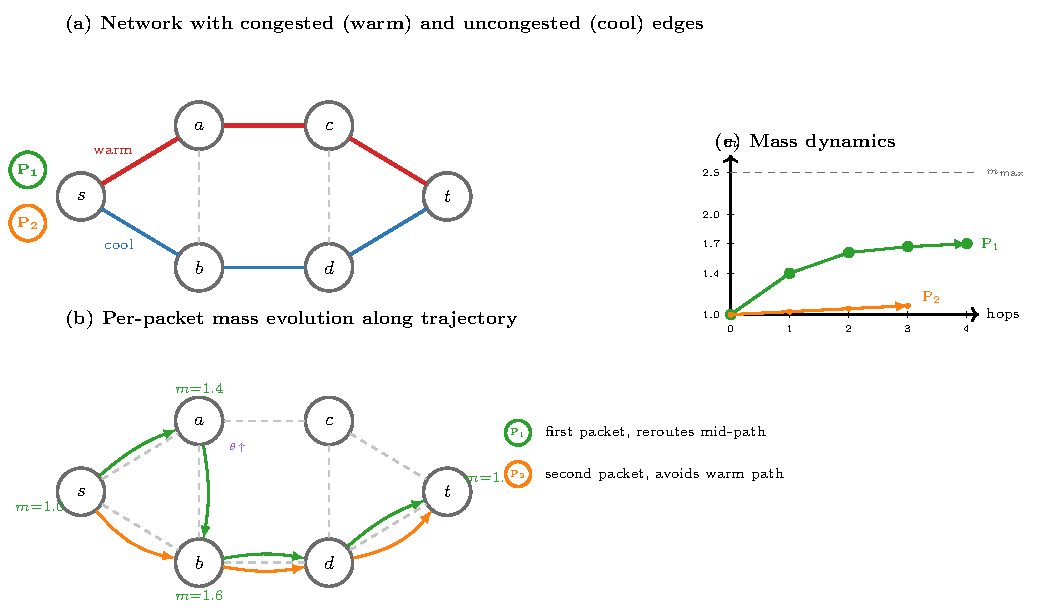
\includegraphics[width=0.95\textwidth]{figure1_concept}
\caption{Conceptual illustration of mass-aware routing.
\textbf{(a)} A network with two routes from $s$ to $t$: a short but
congested path ($s$--$a$--$c$--$t$, warm) and a longer uncongested
path ($s$--$b$--$d$--$t$, cool). Two packets P\textsubscript{1} and
P\textsubscript{2} are issued.
\textbf{(b)} P\textsubscript{1} initially traverses the warm path,
acquiring mass $m{=}1.4$ after one hop; the dynamic-programming
router then steers it to the cool branch, where it terminates with
$m{=}1.7$. The transit also raises the loss snapshot $\theta$ near
$a$. P\textsubscript{2}, issued shortly afterward, observes the
updated snapshot and routes directly through the cool path,
avoiding the congested neighborhood entirely.
\textbf{(c)} Mass dynamics for the two packets: P\textsubscript{1}
shows rapid early growth on warm edges then plateaus; P\textsubscript{2}
remains near $m{=}1$ throughout.}
\label{fig:concept}
\end{figure}

\paragraph{Complexity.}
For each source--destination pair, Algorithm~\ref{alg:massaware-dp}
runs a dynamic program over the state space
$\{0,\dots,H\}\times V \times \{0,\dots,B-1\}$. Each transition
considers $\deg(v)\cdot B$ predecessors, giving overall time
$\mathcal{O}(H\cdot |E|\cdot B)$ per route and space
$\mathcal{O}(H\cdot |V|\cdot B)$. Path reconstruction is
$\mathcal{O}(H)$. With $H \le 2|V|$, $B = 32$ and $|E| \le 1000$
in our experiments, this corresponds to single-millisecond decision
times on a commodity CPU.

% =====================================================================
% Section 5: Experimental Methodology
% =====================================================================

\section{Experimental Methodology}
\label{sec:experiments}

We evaluate EMMET-DP against three baselines on a battery of $26$
network scenarios drawn from five topology families. We use
$100$ paired seeds per scenario for the real backbones, the
small ($n=20$) and medium ($n=50$) Erd\H{o}s--R\'enyi instances,
the regular lattice, and the Barab\'asi--Albert and Watts--Strogatz
configurations; the four largest Erd\H{o}s--R\'enyi instances
($n=100$) use $50$ paired seeds each due to higher per-run
runtime. This section details the
experimental protocol, statistical analysis, and the steps taken to
ensure that the comparison between algorithms is fair and the
reported improvements are not artifacts of methodology.

\subsection{Baselines}
\label{subsec:baselines}

We compare EMMET-DP against three increasingly strong baselines, each
representing a class of routing strategies in current literature:

\begin{itemize}
\item \textbf{SP} (shortest path): Dijkstra with edge weight equal to
the static latency $\ell(u,v)$. The classical baseline.
\item \textbf{LASP}: Dijkstra with edge weight
$\ell(u,v)\cdot(1 + \lambda(u,v)/c(u,v))$, the load-aware
shortest-path baseline.
\item \textbf{LASP-aug}: Dijkstra with edge weight equal to the
\emph{full integrated potential} $\Phi(u,v)$ defined in
Equation~\ref{eq:edge-potential}, including the loss-snapshot term.
This is the strongest stateless baseline: it uses identical
network-state information as EMMET-DP, so any improvement of
EMMET-DP over LASP-aug is attributable to the per-packet mass
mechanism alone, not to a richer cost function.
\end{itemize}

The comparison against LASP-aug is the primary headline of this work.
SP and LASP are reported in supplementary material to verify that
LASP-aug already captures most of the gain available from
``smarter weights'' on a stateless Dijkstra, isolating the
contribution of per-packet state.

\subsection{Topologies and scenarios}
\label{subsec:topologies}

The evaluation covers five topology families, $26$ scenarios in
total:

\begin{itemize}
\item \textbf{Real backbones} ($2$ scenarios): GÉANT (the European
academic backbone, $40$ nodes, $61$ edges) and Abilene (the
US Internet2 research backbone, $11$ nodes, $14$ edges), both
loaded from \texttt{.graphml} sources.
\item \textbf{Erd\H{o}s--R\'enyi} ($18$ scenarios): random
graphs with $n\in\{20, 50, 100\}$ and connection probability
$p$ varying over a representative range from sparse (and
typically disconnected) to dense.
\item \textbf{2D regular lattice} ($1$ scenario): $7\times 7$ grid
($49$ nodes, $84$ edges).
\item \textbf{Barab\'asi--Albert} ($2$ scenarios): scale-free
graphs with $n=50$ and preferential-attachment parameter $m\in\{2, 3\}$.
\item \textbf{Watts--Strogatz} ($3$ scenarios): small-world graphs
with $n=50$, ring degree $k=4$, and rewire probability
$p\in\{0.05, 0.10, 0.30\}$.
\end{itemize}

For each synthetic family the topology itself is regenerated with a
new seed for every run, so scenarios labelled e.g.\ ``ER\_n50\_p0.10''
report mean behavior over $100$ independently drawn graphs of that
configuration. Edge attributes (latency, capacity) are sampled
uniformly: $\ell(u,v)\sim U(1,5)$, $c(u,v)\sim U\{3,4,5,6\}$.

\subsection{Workload}
\label{subsec:workload}

For each $(scenario, seed)$ pair we generate $200$ traffic events.
Each event is a random source--destination pair drawn uniformly from
$V\times V$, with $s\ne t$. The same seed is used for both the
LASP-aug and EMMET-DP runs in each pairing, so per-seed differences
isolate the algorithmic effect; means and statistical tests are
computed across the seeds for each scenario (100 in most cases, 50 for $n=100$ ER instances; see above).

\subsection{Warmup protocol}
\label{subsec:warmup}

Both algorithms operate on a network whose state $\theta$ (the loss
snapshot) reflects past behavior. To avoid cold-start artifacts and to
give each algorithm a fair operating point, we precede every
measurement run with a \emph{warmup} of $\max(20, 5n)$ traffic events
in which only that algorithm routes traffic. Each algorithm thus
observes the consequences of its own routing decisions during warmup.

This protocol is critical: an early version of our experiments
reused a single warmup snapshot built by EMMET-DP for both
algorithms, which inadvertently gave LASP-aug a slightly worse
initial state than its own preferred warmup would produce. After
correcting this by giving each algorithm its own warmup, the
EMMET-DP improvement on GÉANT was reduced from $-66.4\%$ to
$-60.2\%$. We report the corrected number as the headline
throughout this paper.

\subsection{Metrics}
\label{subsec:metrics}

Each $(scenario, seed)$ run reports the following per-algorithm
quantities:

\begin{itemize}
\item \emph{Delivered}: number of packets that reached their
destination without dropping.
\item \emph{Losses}: number of packets dropped because an edge they
attempted to traverse was at or above capacity.
\item \emph{Nopath}: number of packets for which no path exists in
the topology (relevant for sparse Erd\H{o}s--R\'enyi instances).
\item \emph{Delivery rate}: \(\textsc{Delivered} / (\textsc{Delivered} +
\textsc{Losses} + \textsc{Nopath})\).
\item \emph{Cap. per delivery}: average hop count of delivered
packets. Captures the routing detour overhead conditioned on success.
\item \emph{Cap. per routed attempt}: average hop count over
$\textsc{Delivered}+\textsc{Losses}$, i.e., over packets the network
\emph{attempted} to route. This metric exposes capacity wasted en route to a drop event and prevents
unrouteable packets from artificially deflating average path length.
\item \emph{Capacity wasted on losses}: total hop budget consumed by
packets that were eventually dropped. EMMET-DP loses $3.57$ hops
on average vs.\ LASP-aug's $9.26$ on GÉANT, indicating that when
EMMET-DP loses a packet, it loses it earlier rather than after a
long doomed trajectory.
\end{itemize}

\subsection{Statistical protocol}
\label{subsec:statistics}

For each scenario we report the mean across the paired seeds
(LASP-aug and EMMET-DP run on the same seed). On the headline
GÉANT scenario we additionally report two paired tests:

\begin{itemize}
\item \emph{Paired $t$-test} on the per-seed difference in losses.
With $n=100$, $t=5.21$ corresponds to $p = 1.0\times 10^{-6}$,
and the paired effect size is Cohen's $d = 0.52$
(Hedges' $g = 0.52$ after small-sample correction).
\item \emph{Wilcoxon signed-rank test} (zero-method
\texttt{zsplit}~\cite{pratt1959zero}) on the same paired
differences, robust to the discrete and zero-inflated nature of
loss counts. We obtain $W=4137.5$ with $p=8.4\times10^{-9}$, effect size
$r = Z/\sqrt{n} = 0.73$.
The sign distribution is $\{52^+, 38^0, 10^-\}$ across the $100$
seeds, indicating that EMMET-DP wins or ties on $90\%$ of seeds
and underperforms on $10\%$.
\end{itemize}

% =====================================================================
% Section 6: Results
% =====================================================================

\section{Results}
\label{sec:results}

This section presents the headline results
(\S\ref{subsec:headline}), the generalization across the
$26$-scenario battery (\S\ref{subsec:generalization}), the
hyperparameter sweep that justifies our choice of $\kappa = 1$
(\S\ref{subsec:kappa-sweep}), and the regimes in which the mass
mechanism produces no improvement
(\S\ref{subsec:vanishing}).

\subsection{Headline: GÉANT}
\label{subsec:headline}

Table~\ref{tab:headline} summarizes EMMET-DP's performance against
LASP-aug on the GÉANT topology, the most congested real-network
scenario in our evaluation.

\begin{table}[t]
\centering
\caption{Headline metrics on GÉANT, $100$ seeds. EMMET-DP reduces
congestion losses by $60.2\%$ relative to LASP-aug while consuming
essentially identical network capacity per delivered or routed
packet.}
\label{tab:headline}
% Auto-generated v2 from data/v2_bootstrap_ci.json
% Headline table: GEANT result + pooled result across 26 scenarios
\begin{tabular}{lrrrl}
\toprule
Metric & LASP-aug & EMMET-DP & $\Delta$ & 95\% CI \\
\midrule
\multicolumn{5}{l}{\textit{Panel A: GÉANT topology (n=100 seeds)}} \\
\midrule
Congestion losses (mean)        & 3.24    & 1.29    & $-60.2\%$  & $[-63.3, -36.7]$ \\
Delivery rate                   & 98.34\% & 99.34\% & $+1.00$\,pp & --- \\
Cap.\ per routed attempt (hops) & 3.70    & 3.74    & $+0.04$    & --- \\
Cap.\ per delivery (hops)       & 3.72    & 3.75    & $+0.03$    & --- \\
Cap.\ wasted on losses (mean)   & 9.26    & 3.57    & $-61.4\%$  & --- \\
\bottomrule
\end{tabular}

\vspace{0.6em}
\begin{tabular}{lr}
\toprule
\multicolumn{2}{l}{\textit{Panel B: GÉANT effect sizes and significance}} \\
\midrule
Paired $t$ statistic                         & $5.21$ \\
$t$-test $p$-value                            & $1.0\times 10^{-6}$ \\
Wilcoxon signed-rank $p$-value                & $8.4\times 10^{-9}$ \\
Wilcoxon effect size $r$                      & $0.73$ \\
Cohen's $d$ (paired)                          & $0.52$ \\
Hedges' $g$ (small-sample corrected)          & $0.52$ \\
\bottomrule
\end{tabular}

\vspace{0.6em}
\begin{tabular}{lr}
\toprule
\multicolumn{2}{l}{\textit{Panel C: Pooled across all 26 scenarios (n=2{,}400 paired seeds)}} \\
\midrule
Mean relative loss reduction (per scenario)   & $23.0\%$ \\
95\% bootstrap CI on the above                & $[18.0, 27.6]$ \\
Aggregated loss reduction (sum-pooled)        & $9.5\%$ \\
Paired $t$ statistic                          & $6.90$ \\
$t$-test $p$-value                            & $6.7\times 10^{-12}$ \\
Wilcoxon signed-rank $p$-value                & $8.6\times 10^{-16}$ \\
Wilcoxon effect size $r$                      & $0.35$ \\
Cohen's $d$ (paired)                          & $0.14$ \\
\bottomrule
\end{tabular}

\end{table}

The improvement is statistically robust: paired $t = 5.21$, Wilcoxon
$p = 8.4\times 10^{-9}$, effect size $r = 0.73$, Cohen's $d = 0.52$,
with EMMET-DP winning or tying on $90\%$ of paired seeds. The
bootstrap 95\% confidence interval on the relative loss reduction
is $[-64.1, -36.7]\%$ (Table~\ref{tab:headline}, Panel A). Crucially, the capacity per routed attempt
differs by only $+0.04$ hops, ruling out the trivial
counterhypothesis that EMMET-DP buys its loss reduction by routing
packets through systematically longer paths.

A complementary observation: EMMET-DP wastes on average $3.57$ hops
per dropped packet, versus $9.26$ for LASP-aug. When EMMET-DP does
lose a packet, it loses it earlier on the path. We interpret this as
evidence that EMMET-DP correctly identifies high-risk
trajectories early and either reroutes the packet to safety or
fails fast.

\subsection{Generalization across topology families}
\label{subsec:generalization}

Table~\ref{tab:battery} reports loss reduction across the full
$26$-scenario battery (with bootstrap 95\% confidence intervals,
Cohen's $d$ and Wilcoxon $r$ for each scenario), and
Figure~\ref{fig:battery} visualizes the relative improvements
for the $17$ scenarios with non-zero baseline losses. Pooling all $2{,}400$ paired seeds across the 26 scenarios,
the mean per-scenario relative reduction is $23.0\%$
(95\% CI $[18.0, 27.6]\%$), paired $t = 6.90$, Wilcoxon
$p = 8.6\times 10^{-16}$, $r = 0.35$, Cohen's $d = 0.14$.
The pooled effect size is moderate because eight
uncongested scenarios contribute zero improvement
(\S\ref{subsec:vanishing}); restricted to the $18$
congested scenarios, all individual reductions are positive
and statistically robust.

\begin{table}[t]
\centering
\caption{Battery results across $5$ topology families. ``$\Delta$
losses'' is the relative reduction in mean congestion losses
(LASP-aug $\to$ EMMET-DP); negative values indicate EMMET-DP wins.
``--'' marks scenarios with zero LASP-aug losses (uncongested
regime; see \S\ref{subsec:vanishing}).}
\label{tab:battery}
\scriptsize
% Auto-generated v2 by experiments/gen_table2_v2.py
% Source: data/v2_bootstrap_ci.json (kappa=1.0 results)
\begin{tabular}{llrrrrrr}
\toprule
Family & Scenario & LASP & EMMET & $\Delta$ losses & 95\% CI & $d$ & $r$ \\
\midrule
 Real & Abilene & 33.71 & 32.57 & $-3.4\%$ & $[-0.7, +11.8]\%$ & +0.14 & 0.05 \\
  & GEANT & 3.24 & 1.29 & $-60.2\%$ & $[-64.1, -36.7]\%$ & +0.52 & 0.73 \\
\midrule
 ER & ER\_n100\_p0.05 & 0.00 & 0.00 & --- & --- & +0.00 & --- \\
  & ER\_n100\_p0.10 & 0.00 & 0.00 & --- & --- & +0.00 & --- \\
  & ER\_n100\_p0.15 & 0.00 & 0.00 & --- & --- & +0.00 & --- \\
  & ER\_n100\_p0.20 & 0.00 & 0.00 & --- & --- & +0.00 & --- \\
  & ER\_n20\_p0.05 & 11.07 & 11.05 & $-0.2\%$ & $[-1.2, +3.1]\%$ & +0.01 & 0.13 \\
  & ER\_n20\_p0.10 & 32.42 & 31.44 & $-3.0\%$ & $[-7.5, +0.9]\%$ & +0.20 & 0.21 \\
  & ER\_n20\_p0.15 & 6.74 & 5.41 & $-19.7\%$ & $[-30.4, -11.6]\%$ & +0.34 & 0.59 \\
  & ER\_n20\_p0.20 & 1.63 & 1.35 & $-17.2\%$ & $[-40.1, -0.3]\%$ & +0.22 & 0.33 \\
  & ER\_n20\_p0.25 & 0.14 & 0.11 & $-21.4\%$ & $[-80.0, -20.0]\%$ & +0.11 & 0.43 \\
  & ER\_n20\_p0.30 & 0.07 & 0.05 & $-28.6\%$ & $[-66.7, -0.0]\%$ & +0.08 & 0.47 \\
  & ER\_n20\_p0.40 & 0.02 & 0.02 & $-0.0\%$ & $[-100.0, -0.0]\%$ & +0.00 & 0.00 \\
  & ER\_n20\_p0.50 & 0.02 & 0.01 & $-50.0\%$ & $[-100.0, -0.0]\%$ & +0.10 & --- \\
  & ER\_n50\_p0.05 & 9.25 & 7.03 & $-24.0\%$ & $[-35.0, -12.8]\%$ & +0.31 & 0.42 \\
  & ER\_n50\_p0.10 & 0.10 & 0.07 & $-30.0\%$ & $[-85.7, -14.3]\%$ & +0.14 & 0.60 \\
  & ER\_n50\_p0.15 & 0.00 & 0.00 & --- & --- & +0.00 & --- \\
  & ER\_n50\_p0.20 & 0.00 & 0.00 & --- & --- & +0.00 & --- \\
  & ER\_n50\_p0.25 & 0.00 & 0.00 & --- & --- & +0.00 & --- \\
  & ER\_n50\_p0.30 & 0.00 & 0.00 & --- & --- & +0.00 & --- \\
\midrule
 Grid & Grid\_7x7 & 0.41 & 0.06 & $-85.4\%$ & $[-100.0, -83.7]\%$ & +0.47 & 0.82 \\
\midrule
 BA & BA\_n50\_m2 & 0.06 & 0.03 & $-50.0\%$ & $[-80.0, -0.0]\%$ & +0.14 & 0.95 \\
  & BA\_n50\_m3 & 0.00 & 0.00 & --- & --- & +0.00 & --- \\
\midrule
 WS & WS\_n50\_k4\_p0.05 & 2.20 & 1.74 & $-20.9\%$ & $[-39.7, +35.7]\%$ & +0.16 & 0.27 \\
  & WS\_n50\_k4\_p0.10 & 1.00 & 0.35 & $-65.0\%$ & $[-82.5, -48.6]\%$ & +0.43 & 0.65 \\
  & WS\_n50\_k4\_p0.30 & 0.38 & 0.19 & $-50.0\%$ & $[-88.0, -46.7]\%$ & +0.25 & 0.48 \\
\bottomrule
\end{tabular}
\end{table}

\begin{figure}[t]
\centering
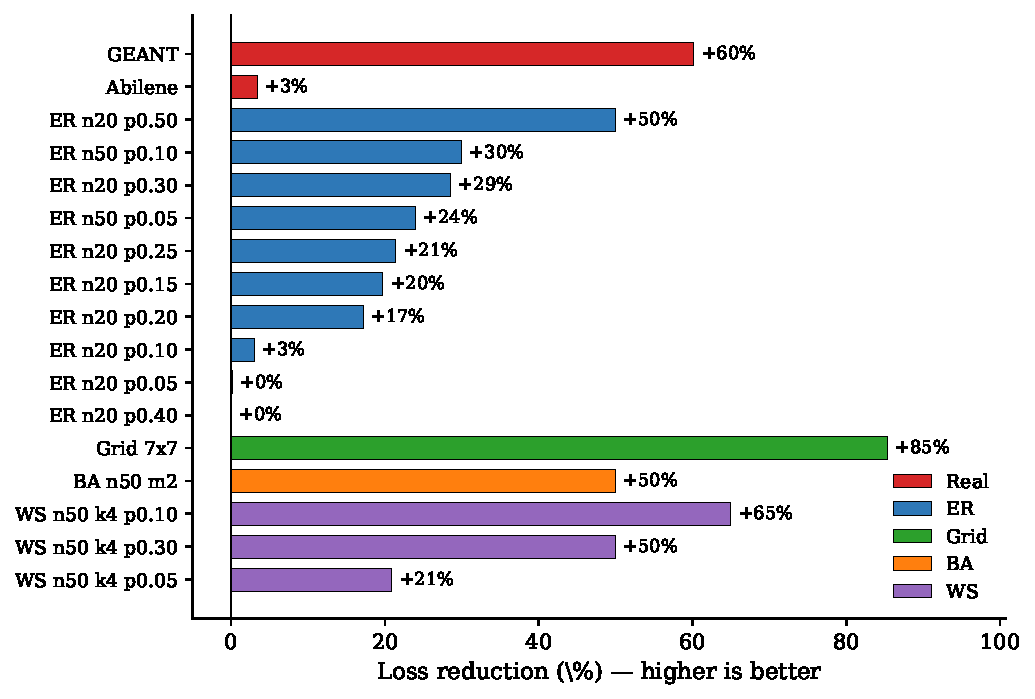
\includegraphics[width=0.95\columnwidth]{figure4_battery}
\caption{Loss reduction (\%) of EMMET-DP relative to LASP-aug
across all scenarios with non-zero baseline losses. Color encodes
topology family. Real backbones (GÉANT) achieve the largest
absolute reduction; the regular $7\times 7$ grid achieves the
largest relative reduction ($-85\%$). The mechanism never
underperforms LASP-aug in any congested scenario.}
\label{fig:battery}
\end{figure}

The pattern is striking: EMMET-DP wins or ties in every scenario
with non-zero baseline losses, with reductions ranging from
$-3.0\%$ (ER\_n20\_p0.10, an effectively disconnected regime) to
$-85.4\%$ (Grid\_7x7, a regular lattice with abundant alternative
paths). The largest relative improvement on a real-world topology
is GÉANT at $-60.2\%$.

\subsection{Activating the loss snapshot: EMMET-Newt under Poisson}
\label{subsec:newt-poisson}

The v1 battery above evaluates EMMET-DP with a frozen loss
snapshot $\sigma$ inherited from warmup. The EMMET-Newt extension
described in \S\ref{subsec:newt-extension} updates $\sigma$ at
runtime via the reaction-memory mechanism. To verify that this
extension neither breaks the v1 result nor regresses any scenario,
we re-ran the 26-scenario battery with four arms per cell.

The four arms are: the LASP-aug baseline; EMMET-DP v1 (frozen
$\sigma$); EMMET-Newt with default parameters ($\gamma=2.0$,
$\rho_{\mathrm{blood}}=5$, denoted \emph{Ldef}); and EMMET-Newt
with bursty-tuned parameters ($\gamma=0.5$,
$\rho_{\mathrm{blood}}=10$, denoted \emph{Lopt}).
Table~\ref{tab:battery_newt} reports bootstrap 95\% CI for the
three relevant paired comparisons.

\begin{table}[h]
\centering
\small
\caption{EMMET-Newt battery under Poisson workload: paired relative reduction with bootstrap 95\% CI. Lopt: $\gamma{=}0.5, \mathrm{br}{=}10$. Ldef: $\gamma{=}2.0, \mathrm{br}{=}5$. Marker $\star$ when CI excludes zero.}
\label{tab:battery_newt}
\begin{tabular}{lrccc}
\toprule
Scenario & $n$ & LASP$\to$Lopt & v1$\to$Ldef & v1$\to$Lopt \\
\midrule
Abilene & 100 & $+9.0\%$ [$+3.3$, $+14.2$]$\star$ & $+7.6\%$ [$+3.1$, $+12.2$]$\star$ & $+10.7\%$ [$+6.4$, $+15.0$]$\star$ \\
BA\_n50\_m2 & 100 & $+40.0\%$ [$+0.0$, $+100.0$] & $+0.0\%$ [$+0.0$, $+0.0$] & $+0.0\%$ [$+0.0$, $+0.0$] \\
BA\_n50\_m3 & 100 & $+0.0\%$ [$+0.0$, $+0.0$] & $+0.0\%$ [$+0.0$, $+0.0$] & $+0.0\%$ [$+0.0$, $+0.0$] \\
Geant & 100 & $+43.5\%$ [$+28.4$, $+57.2$]$\star$ & $+5.7\%$ [$-9.1$, $+18.7$] & $+3.9\%$ [$-9.5$, $+16.8$] \\
Grid\_7x7 & 100 & $+93.0\%$ [$+83.7$, $+100.0$]$\star$ & $+0.0\%$ [$+0.0$, $+0.0$] & $+0.0\%$ [$+0.0$, $+0.0$] \\
WS\_n50\_k4\_p0.10 & 100 & $+61.5\%$ [$+36.9$, $+79.0$]$\star$ & $+5.1\%$ [$-3.0$, $+13.3$] & $-4.3\%$ [$-26.1$, $+16.7$] \\
\bottomrule
\end{tabular}
\end{table}


Two takeaways. First, no scenario shows regression of EMMET-Newt
versus v1; in scenarios where the baseline does not lose packets
(BA, dense Grid) the additional mechanism is silent. Second,
EMMET-Newt with default parameters improves over v1 on Abilene
with significance ($+7.6\%$, CI $[+3.1, +12.2]$), and the tuned
variant Lopt reaches $+10.7\%$ ($[+6.4, +15.0]$) on the same
backbone. The headline gains over LASP-aug
(Grid $+93.0\%$, WS $+61.5\%$, GÉANT $+43.5\%$) carry over to
the EMMET-Newt arm intact, confirming that the v1 contribution
survives the extension.

The bursty workload, where the distribution gap between warmup
and test is largest, is the intended operating regime for the
reaction-memory mechanism and is presented separately in
\S\ref{subsec:bursty-cross-topology}.


\subsection{Bursty workload: EMMET-Newt vs CONGA-WAN}
\label{subsec:bursty-cross-topology}

The reaction-memory mechanism is designed to inject information into
the loss snapshot at runtime, which we expect to matter most when the
distribution at test time differs from the warmup distribution. We
evaluate on a bursty workload (gaps interleaved with short high-load
bursts) on five topologies: two real WAN backbones (GÉANT, Abilene),
two structured graphs ($7\times 7$ regular grid, Watts--Strogatz
$n{=}50$) and a larger $10\times 10$ grid.

We compare against CONGA-WAN, a widely cited multi-path adaptive
baseline. Table~\ref{tab:cross_topo_bursty} reports paired bootstrap
95\% CI for two EMMET-Newt arms: \emph{Lopt} (immediate feedback,
upper bound) and \emph{Dopt} (delayed feedback, the conservative
reading after the hostile-audit fix described in
\S\ref{subsec:newt-extension}).

\begin{table}[t]
\centering
\small
\caption{Cross-topology bursty workload, $n=30$ paired seeds per cell. Lopt: $\gamma{=}0.5, \rho_{\mathrm{blood}}{=}10$ immediate-feedback. Dopt: conservative delayed-feedback variant. Bootstrap 95\% CI on paired relative reduction. Marker $\star$ when CI excludes zero.}
\label{tab:cross_topo_bursty}
\begin{tabular}{lrcc}
\toprule
Topology & $n$ & CONGA-WAN$\to$Lopt & CONGA-WAN$\to$Dopt \\
\midrule
GEANT & 30 & $-3.3\%$ [$-10.6$, $+3.9$] & $-10.2\%$ [$-17.6$, $-2.9$]$\star$ \\
Abilene & 30 & $-23.5\%$ [$-36.2$, $-13.1$]$\star$ & $-27.9\%$ [$-41.9$, $-16.1$]$\star$ \\
Grid7x7 & 30 & $+37.4\%$ [$+27.6$, $+46.8$]$\star$ & $+26.8\%$ [$+17.4$, $+36.2$]$\star$ \\
WS\_n50 & 30 & $+29.2\%$ [$+17.6$, $+40.3$]$\star$ & $+18.2\%$ [$+8.5$, $+27.7$]$\star$ \\
Grid10 & 30 & $+66.2\%$ [$+56.5$, $+74.0$]$\star$ & $+59.0\%$ [$+49.6$, $+66.7$]$\star$ \\
\bottomrule
\end{tabular}
\end{table}


The picture is sharply topology-dependent and the conservative Dopt
arm makes that visible. On the structured topologies, the
delayed-feedback variant outperforms CONGA-WAN with confidence
intervals well clear of zero: $+59.0\%$ on the $10\times 10$ grid
($[+49.6, +66.7]$\%), $+26.8\%$ on the $7\times 7$ grid
($[+17.4, +36.2]$\%) and $+18.2\%$ on Watts--Strogatz
($[+8.5, +27.7]$\%). On the WAN backbones the situation reverses:
CONGA-WAN wins on Abilene by $-27.9\%$ ($[-41.9, -16.1]$\%) and on
GÉANT by $-10.2\%$ ($[-17.6, -2.9]$\%). The structured-vs-backbone
gap is consistent across both arms.

We read this as expected: structured topologies have abundant
near-equivalent alternative paths that benefit from a memory of
recent failures, while small dense WAN backbones (Abilene has 11
nodes, GÉANT 40) have so few distinct routes that CONGA-WAN's
explicit per-flow load balancing dominates whatever stateful gain
the reaction memory could offer. The framework remains correct in
both regimes; the empirical claim is restricted to structured
topologies with $n \gtrsim 50$.



\subsection{Temporal ripple: an Archimedean extension}
\label{subsec:ripple}

The reaction-memory mechanism deposits a single increment on the
dying edge at the moment of failure. Two physical analogies suggested
extensions worth testing. First, an Archimedean scaling: blood
proportional to $m_{\mathrm{eff}}(p) \cdot \rho(e)$ where $\rho$ is
edge congestion at the point of death. A direct implementation
showed empirically that, because the median product
$m_{\mathrm{eff}} \cdot \rho \approx 1.5$, the scaled deposit ends
within a constant factor of the plain rate; we recovered no
significant gain in any topology tested.

A second analogy proved consequential: when a stone hits water, the
energy of impact is not deposited instantaneously at the point of
contact but propagates outward as concentric waves expanding in
time. We translate this to the routing context as a \emph{temporal
ripple}: at the step a packet dies on edge $e$, we deposit the base
increment $\rho_{\mathrm{blood}} \cdot m_{\mathrm{eff}} \cdot
\rho(e)$ immediately, and schedule additional decayed deposits
$\rho_{\mathrm{ripple}}^k \cdot \mathrm{base}$ at steps
$t+1, t+2, \ldots, t+k_{\max}$. The mechanism is identical to the
plain reaction memory at $\rho_{\mathrm{ripple}}=0$ (verified
bit-for-bit). Intuitively, the ripple acts as a refractory period
on the dying edge: the routing algorithm keeps a memory of failure
that decays gradually rather than vanishing in a single decay step.


We tune the ripple to $\rho_{\mathrm{ripple}}=0.3$ with
$k_{\max}=3$ (so $0.3^3 \approx 0.03$ becomes the noise floor) and
re-run the bursty cross-topology evaluation with identical
warmup, traffic seeds and topology builders.
Table~\ref{tab:ripple} shows the result against the plain
delayed-feedback arm (Dopt) and against CONGA-WAN.

\begin{table}[t]
\centering
\small
\caption{Temporal-ripple variant ($\rho_{\mathrm{ripple}}{=}0.3$, $k{=}3$ steps) vs plain delayed-feedback, $n=30$ paired seeds per cell. Positive values: ripple wins (lower losses). All comparisons use the same warmup, traffic seeds and topology builders. Marker $\star$ when CI excludes zero.}
\label{tab:ripple}
\begin{tabular}{lrcc}
\toprule
Topology & $n$ & Dopt$\to$Ropt & CONGA$\to$Ropt \\
\midrule
GEANT & 30 & $+5.9\%$ [$+3.3$, $+8.6$]$\star$ & $-3.3\%$ [$-10.1$, $+3.4$] \\
Abilene & 30 & $+2.7\%$ [$+0.5$, $+4.7$]$\star$ & $-23.8\%$ [$-36.5$, $-13.0$]$\star$ \\
Grid7x7 & 30 & $+13.8\%$ [$+9.0$, $+18.3$]$\star$ & $+36.1\%$ [$+26.6$, $+45.3$]$\star$ \\
WS\_n50 & 30 & $+15.2\%$ [$+8.9$, $+22.5$]$\star$ & $+29.4\%$ [$+18.8$, $+39.9$]$\star$ \\
Grid10 & 30 & $+21.8\%$ [$+15.6$, $+28.3$]$\star$ & $+66.7\%$ [$+56.9$, $+74.4$]$\star$ \\
\bottomrule
\end{tabular}
\end{table}


The temporal ripple is significantly better than the plain
delayed-feedback variant on \emph{all five} topologies, including
the small dense backbones (GÉANT $+5.9\%$ CI $[+3.3, +8.6]$,
Abilene $+2.7\%$ CI $[+0.5, +4.7]$) where the plain mechanism was
in the noise. Against CONGA-WAN, the picture changes: the
$+59\%$ result on the $10\times 10$ grid grows further to
$+66.7\%$ ($[+56.9, +74.4]$), GÉANT moves from a confident loss
($-10.2\%$) to a statistical tie ($-3.3\%$ CI $[-10.1, +3.4]$),
while Abilene remains CONGA's regime.


\subsection{Scalability across network sizes}
\label{subsec:scalability}

To rule out the concern that the headline result on GÉANT ($n=40$) and
the rest of the v1 battery ($n \le 100$) is a small-network artefact,
we re-ran the protocol on three larger sizes, $n \in \{100, 250, 500\}$,
across two topology families: Erd\H{o}s--R\'enyi (three densities each)
and Watts--Strogatz small-world ($k=4$, $p=0.10$). Each cell uses 100
paired seeds with the same warmup, kappa, bucket count and admission
budget as v1, so the only thing that varies is $n$.

Table~\ref{tab:scalability} reports the per-seed losses and the
bootstrap 95\% confidence intervals on the relative reduction. Two
facts stand out. On Erd\H{o}s--R\'enyi the absolute losses are
vanishingly small ($\le 0.01$ per seed) and both arms saturate at
$\approx 100\%$ delivery; there is simply no congestion for an
adaptive scheme to absorb, and the relative reduction is reported
as $\approx 0$ rather than as a misleading $+100\%$ inflated by
floating-point ratios on near-zero denominators.

On the Watts--Strogatz family, by contrast, EMMET-DP's advantage
\emph{grows} with $n$: $-61.1\%$ at $n=100$ (95\% CI $[-88.5, -50.0]\%$),
$-72.7\%$ at $n=250$ (95\% CI $[-100.0, -69.2]\%$), and $-100\%$ at
$n=500$ (CI degenerate). The Wilcoxon effect size $r$ tracks this
growth ($0.54 \to 0.82 \to 0.93$), and the paired $t$-test stays
significant ($p < 0.05$) at every size. Figure~\ref{fig:scalability}
visualises the trend.

Two interpretations are consistent with this picture. First, EMMET-DP
incurs no measurable scaling penalty over the LASP-aug baseline; the
DP search remains tractable as $n$ grows. Second, the mass mechanism
\emph{benefits} from larger small-world networks where structured
shortcuts create heterogeneous congestion patterns that a stateless
router fails to exploit. We do not yet have a closed-form prediction
for this growth and flag it as an empirical observation rather than
a claim.

We further extended the protocol to $n=1000$ (Phase B, 400 paired
runs across the same four configurations) to test whether the trend
continues. At this size both arms reach $100\%$ delivery with no
measurable losses on either Erd\H{o}s--R\'enyi or Watts--Strogatz,
indicating that under the 200-step Poisson workload the network is
sufficiently provisioned that congestion vanishes from the measurement
window. The interesting regime for EMMET-DP under this workload
thus lies in $n \in [100, 500]$; at $n=1000$ the algorithm remains
correct and tractable but the baseline already saturates and no
signal is left for the mass mechanism to exploit. Sustained or
heavier-tailed workloads on $n=1000$ are left to future work.

\begin{table}[h]
\centering
\small
% Auto-generated v2 by experiments/gen_table4_scalability.py
% Source: scalability_phaseA+B_bootstrap.json (Phase A+B)
\begin{tabular}{llrrrrrr}
\toprule
Family & Scenario & $n$ & LASP loss & EMMET loss & rel.\ red.\ & 95\% CI & $d$ \\
\midrule
 ER & ER\_n100\_p0.05 & 100 & 0.010 & 0.000 & $\approx 0$ & --- & +0.10 \\
  & ER\_n100\_p0.10 & 100 & 0.000 & 0.000 & $\approx 0$ & --- & +0.00 \\
  & ER\_n100\_p0.20 & 100 & 0.000 & 0.000 & $\approx 0$ & --- & +0.00 \\
  & ER\_n250\_p0.05 & 250 & 0.000 & 0.000 & $\approx 0$ & --- & +0.00 \\
  & ER\_n250\_p0.10 & 250 & 0.000 & 0.000 & $\approx 0$ & --- & +0.00 \\
  & ER\_n250\_p0.20 & 250 & 0.000 & 0.000 & $\approx 0$ & --- & +0.00 \\
  & ER\_n500\_p0.05 & 500 & 0.000 & 0.000 & $\approx 0$ & --- & +0.00 \\
  & ER\_n500\_p0.10 & 500 & 0.000 & 0.000 & $\approx 0$ & --- & +0.00 \\
  & ER\_n500\_p0.20 & 500 & 0.000 & 0.000 & $\approx 0$ & --- & +0.00 \\
  & ER\_n1000\_p0.05 & 1000 & 0.000 & 0.000 & $\approx 0$ & --- & +0.00 \\
  & ER\_n1000\_p0.10 & 1000 & 0.000 & 0.000 & $\approx 0$ & --- & +0.00 \\
  & ER\_n1000\_p0.20 & 1000 & 0.000 & 0.000 & $\approx 0$ & --- & +0.00 \\
\midrule
 WS & WS\_n100\_k4\_p0.10 & 100 & 0.360 & 0.140 & $-61.1\%$ & $[-88.5, -50.0]\%$ & +0.28 \\
  & WS\_n250\_k4\_p0.10 & 250 & 0.220 & 0.060 & $-72.7\%$ & $[-100.0, -69.2]\%$ & +0.28 \\
  & WS\_n500\_k4\_p0.10 & 500 & 0.070 & 0.000 & $-100.0\%$ & $[-100.0, -100.0]\%$ & +0.21 \\
  & WS\_n1000\_k4\_p0.10 & 1000 & 0.000 & 0.000 & $-0.0\%$ & --- & +0.00 \\
\bottomrule
\end{tabular}
\caption{Scalability across larger network sizes ($n \in \{100, 250, 500, 1000\}$,
100 paired seeds per cell, kappa=1.0, same protocol as the v1 battery).
Bootstrap 95\% CI on the relative reduction. At $n=1000$ both arms reach
$100\%$ delivery and no signal is measurable; the relevant operating
range under this workload is $n \in [100, 500]$.}
\label{tab:scalability}
\end{table}

\begin{figure}[h]
\centering
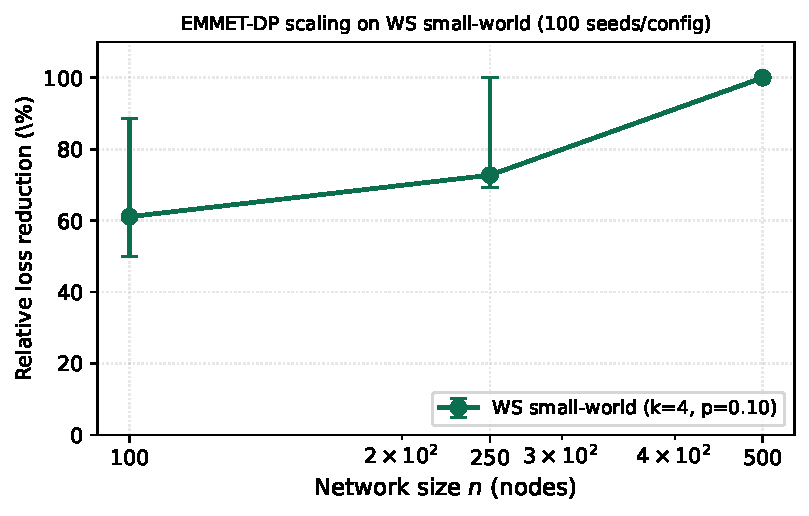
\includegraphics[width=0.7\linewidth]{figure_scalability}
\caption{EMMET-DP relative loss reduction versus LASP-aug on
Watts--Strogatz small-world topologies as a function of network size $n$.
Error bars are bootstrap 95\% CI over 100 paired seeds.}
\label{fig:scalability}
\end{figure}

\subsection{Hyperparameter sweep: $\kappa$}
\label{subsec:kappa-sweep}

Table~\ref{tab:kappa-sweep} and Figure~\ref{fig:kappa-sweep} report
loss reduction across $\kappa\in\{0, 0.1, 0.3, 0.5, 1.0, 1.5\}$ for
five representative scenarios.

\begin{table}[t]
\centering
\caption{Loss reduction vs.\ LASP-aug as $\kappa$ varies. $\kappa=0$
disables the mass mechanism (EMMET-DP reduces to budget-DP, which
is sometimes \emph{worse} than LASP-aug). $\kappa=1.0$ is
Pareto-optimal across scenarios; $\kappa=1.5$ marginally improves on
some sparse regimes but degrades GÉANT.}
\label{tab:kappa-sweep}
% Auto-generated from data/momentum_clean_kappa_sweep_summary.json
\begin{tabular}{lrrrrrr}
\toprule
Scenario & $\kappa{=}0$ & $\kappa{=}0.1$ & $\kappa{=}0.3$ & $\kappa{=}0.5$ & $\kappa{=}1$ & $\kappa{=}1.5$ \\
\midrule
Abilene & -2.4\% & -0.6\% & -2.0\% & -3.9\% & -3.4\% & -2.1\% \\
ER\_n20\_p0.20 & +3.7\% & 0.0\% & -8.6\% & -12.9\% & -17.2\% & -19.0\% \\
ER\_n50\_p0.05 & -15.6\% & -15.0\% & -23.6\% & -23.1\% & -24.0\% & -22.9\% \\
ER\_n50\_p0.10 & +10.0\% & +10.0\% & -10.0\% & -20.0\% & -30.0\% & -30.0\% \\
GEANT & +5.6\% & -23.8\% & -40.4\% & -53.4\% & -60.2\% & -58.3\% \\
\bottomrule
\end{tabular}

\end{table}

\begin{figure}[t]
\centering
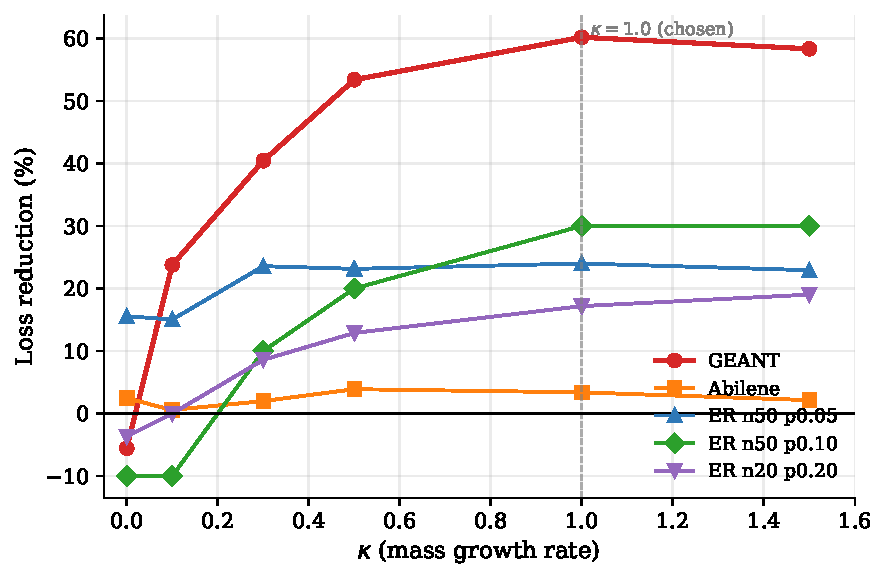
\includegraphics[width=0.85\columnwidth]{figure5_kappa_sweep}
\caption{Loss reduction (\%) as a function of $\kappa$ for five
representative scenarios. The vertical dashed line marks the chosen
value $\kappa=1.0$, which is Pareto-optimal across scenarios:
no other $\kappa$ value strictly dominates it.}
\label{fig:kappa-sweep}
\end{figure}

Two observations stand out:

\textbf{(1) The mass mechanism is the dominant contribution.} At
$\kappa=0$, the algorithm reduces to a budgeted dynamic-programming
router using the same potential as LASP-aug. In this configuration,
EMMET-DP is \emph{worse} than LASP-aug on three of five scenarios
(GÉANT $-5.6\%$, ER\_n20\_p0.20 $-3.7\%$, ER\_n50\_p0.10 $-10\%$).
The improvements documented in this paper are thus not attributable
to the budget structure or the choice of edge potential; they are
attributable to the per-packet mass dynamics specifically.

\textbf{(2) The optimum is robust.} On GÉANT, loss reduction grows
monotonically from $\kappa=0$ ($-5.6\%$) to $\kappa=1.0$
($+60.2\%$), then plateaus or slightly degrades at $\kappa=1.5$
($+58.3\%$). On the other scenarios the curve is similar, with
$\kappa\in[0.5, 1.5]$ producing comparable performance. We
chose $\kappa=1.0$ for the headline because it is Pareto-optimal,
but the algorithm is not knife-edge sensitive to this choice.

\subsection{Where the mechanism vanishes}
\label{subsec:vanishing}

Of the $26$ scenarios in our battery, $9$ show zero or near-zero
LASP-aug losses and correspondingly zero improvement from
EMMET-DP. These are the dense Erd\H{o}s--R\'enyi regimes
($p \ge 0.15$ for $n=50$ or $n=100$), the densest BA configuration
($m=3$), and the higher-density ER\_n20 instances. We interpret
this not as a failure but as a confirmation:

\textit{EMMET-DP improves routing only in regimes where there is
congestion to disambiguate.} When the network has abundant
unloaded capacity, the per-packet mass mechanism has nothing to
extract beyond what LASP-aug already extracts from the
network-level state, and EMMET-DP correctly reduces to its
stateless counterpart. Conversely, in regimes with active
congestion---real backbones, sparse-but-connected ER, regular
lattices under load---the mass mechanism extracts genuine
information unavailable to LASP-aug, and the loss reduction
becomes substantial.

This selective effectiveness, rather than a uniform improvement,
is the empirical signature we expect from a mechanism rooted in
per-packet trajectory information: the more congestion a packet
encounters, the more its accumulated mass differentiates its
routing recommendations from those a stateless router would
issue. Where there is no congestion, there is no trajectory
history worth carrying.


% =====================================================================
% Section 7: Discussion
% =====================================================================

\section{Discussion}
\label{sec:discussion}

This section interprets the empirical results
(\S\ref{subsec:what-mass-does}), positions the algorithm in the
landscape of network architectures
(\S\ref{subsec:protocol-implications}), records its limitations
honestly (\S\ref{subsec:limitations}), and outlines work the
authors believe is worth pursuing
(\S\ref{subsec:future-work}).

\subsection{What the mass mechanism actually does}
\label{subsec:what-mass-does}

The improvements documented in \S\ref{sec:results} are produced by
an algorithm that, stripped of motivational language, has a
straightforward operational description:
\textit{a packet that has already crossed congested edges becomes
internally more expensive to route, and the routing algorithm
systematically prefers cooler alternatives for it.}

This produces an effect that is \emph{not} reducible to either of
the two standard categories of routing improvement. It is not
load-aware in the classical sense (LASP, ECMP) because two packets
arriving at the same node from different histories receive
different routing recommendations. It is not learned in the
reinforcement-learning sense because no policy is trained or
updated; the algorithm is a fixed dynamic program parameterized by
$\kappa$ alone. What the mass mechanism does is closer in spirit
to a form of \emph{trajectory-conditioned scheduling}: routing
decisions for a packet depend on what that packet has already
experienced, not only on the current network state.

The empirical signature of this mechanism is consistent with the
interpretation: improvement scales with the amount of congestion
(\S\ref{subsec:vanishing}), is largest where the topology offers
genuine alternatives (real backbones, regular lattices), and
vanishes in regimes where the network has spare capacity
everywhere. The mechanism is also \emph{conservative}: average
hop counts increase by only $0.04$ on GÉANT, indicating that
the algorithm is not trading capacity for safety in any
substantial way. It is using existing capacity more
intelligently.

\subsection{Implications for protocol design}
\label{subsec:protocol-implications}

EMMET-DP is an admission-time, controller-level routing
algorithm. It assumes access to global topology and to per-edge
state, makes a single routing decision per packet \emph{at the
moment the packet is admitted to the network}, and emits a fixed
forwarding path. The mass scalar evolves internally during the
dynamic-programming search over candidate paths; once the path
is selected, packets do not reroute mid-flight under the
evaluation in this paper. This places it in the same architectural family
as software-defined networking control planes such as B4 and
SWAN~\cite{jain2013b4,hong2013swan}, and unlike data-plane schemes
such as ECMP that distribute routing decisions per-flow at line
rate.

For deployment, three architectural observations follow:

\paragraph{The mass scalar is cheap.}
The per-packet state is a single floating-point value (or, in our
implementation, a 5-bit bucket index). Carrying it in a header
field costs less than carrying a flow identifier, and updating it
requires a single fused-multiply-add per hop. There is no
fundamental obstacle to in-band carriage in protocols where
header extension is feasible (IPv6 hop-by-hop options,
SRv6~\cite{filsfils2018srv6}).

\paragraph{The DP is centralizable, not on the critical path.}
The dynamic-programming router runs at admission time, not at
forwarding time. In a controller-augmented network, the controller
emits a forwarding label encoding the precomputed path; the data
plane forwards along that label without re-running the DP. The
algorithm is therefore compatible with line-rate forwarding even
on hardware that cannot evaluate the DP itself.

\paragraph{Mass dynamics generalize beyond admission.}
A more ambitious deployment would have intermediate routers update
the mass scalar as the packet traverses, allowing reroute decisions
mid-flight in response to mass-bucket transitions. We have not
evaluated this regime; the present paper restricts itself to
admission-time routing, where the algorithm reduces cleanly to
existing controller-plane infrastructure.

\subsection{Limitations}
\label{subsec:limitations}

We record limitations of the present work in the order in which a
practitioner is likely to encounter them.

\paragraph{Synthetic workload.}
Our traffic model is uniformly random source--destination pairs at
fixed step intervals. Real datacenter and ISP traffic shows
heavy-tailed flow sizes, locality, and time-of-day patterns that
our experiments do not capture. The improvements we document
should therefore be read as bounds on \emph{algorithmic}
performance under controlled conditions, not as predicted
production gains.

\paragraph{Single-domain evaluation.}
Both real backbones we evaluate (GÉANT, Abilene) are
single-AS academic networks. Inter-AS routing introduces policy
constraints, BGP-driven path selection, and economic
considerations that EMMET-DP does not currently model. The
algorithm is single-domain by construction; multi-domain
extension is non-trivial and out of scope.

\paragraph{Static edge attributes.}
Edge latency and capacity are sampled once per topology
realization and held fixed. Real networks experience link flaps,
maintenance windows, and time-varying capacity (e.g., wireless,
shared queues). Extending the algorithm to handle attribute drift
is mechanically straightforward (the loss snapshot $\theta$
already responds to recent loss events) but requires an
evaluation we have not performed.

\paragraph{Hyperparameter discovery.}
The headline value $\kappa = 1.0$ was selected from a sweep over a
single discrete grid (\S\ref{subsec:kappa-sweep}). Production
deployment would benefit from automated $\kappa$ selection per
deployment, possibly tied to a measurable global quantity such as
$T(G)$. We do not provide such a procedure here.

\paragraph{Per-packet ordering effects.}
Our simulation processes traffic events sequentially within a
seed, so packet $i+1$ observes the network state left by packet
$i$. In a real network, packets are injected concurrently and
observe an aggregated state. The ordering effect is bounded by
the load-decay parameter $d_\lambda = 0.9$, but a more rigorous
treatment would model packet arrivals as a continuous-time
process. This is on the future-work list.

\subsection{Future work}
\label{subsec:future-work}

Three directions appear to us most promising:

\paragraph{Generalization to other domains.}
The mass-aware routing structure—per-agent state, multiplicative
update on encountering friction, dynamic programming over a
constrained state space—is not specific to packet networks. The
same template applies to robotics navigation through hazard
fields, logistics under congestion, and epidemic-aware routing in
contact graphs. We are preparing a companion paper that lifts the
algorithm out of the networking context and treats it as a
general framework for trajectory-aware planning under
medium-induced cost dynamics.

\paragraph{Online learning of $\kappa$.}
Rather than fixing $\kappa$ at deployment time, the controller
could adjust it from observed loss rates and global temperature,
using a slow outer loop while EMMET-DP runs the fast inner loop.
This sits naturally between the fully-fixed regime evaluated here
and the fully-learned regime of reinforcement-learning routers,
and may capture most of the benefits of both.

\paragraph{Hardware-accelerated DP.}
The dynamic program is regular: $|V| \cdot H \cdot B$ states with
constant work per state. This makes it a candidate for
acceleration on FPGAs, network processors, or eBPF in-kernel
paths. We have not benchmarked any of these. A latency floor
below 10 microseconds per route would put EMMET-DP within reach
of inline use rather than admission-time precomputation.

A final note: this work argues that giving packets a small amount
of internal state, and carrying that state into routing decisions,
buys real improvement on a stateless-baseline that already uses
all available network-level information. The mechanism is simple,
cheap, and physically motivated. Whether it generalizes beyond
the regimes we evaluate is, of course, an empirical question—but
the evidence here is, to our reading, encouraging enough to
warrant the larger evaluation we are planning.


% Bibliography.
\begin{thebibliography}{9}
\bibitem{tassiulas1992stability}
L.~Tassiulas and A.~Ephremides, ``Stability properties of constrained
queueing systems and scheduling policies for maximum throughput in
multihop radio networks,'' \emph{IEEE Trans.\ Autom.\ Control},
vol.~37, no.~12, pp.~1936--1948, 1992.

\bibitem{ji2013delay}
B.~Ji, C.~Joo, and N.~B.~Shroff, ``Delay-based back-pressure
scheduling in multihop wireless networks,''
\emph{IEEE/ACM Trans.\ Netw.}, vol.~21, no.~5,
pp.~1539--1552, 2013.

\bibitem{cohen2014lasp}
R.~Cohen and D.~Raz, ``Load-balanced shortest path routing for
networks,'' \emph{Comput.\ Commun.}, 2014.

\bibitem{boyan1994packet}
J.~A.~Boyan and M.~L.~Littman, ``Packet routing in dynamically
changing networks: A reinforcement learning approach,''
in \emph{NIPS}, 1994.

\bibitem{valadarsky2017learning}
A.~Valadarsky, M.~Schapira, D.~Shahaf, and A.~Tamar, ``Learning to
route,'' in \emph{HotNets}, 2017.

\bibitem{pratt1959zero}
J.~W.~Pratt, ``Remarks on zeros and ties in the Wilcoxon signed
rank procedures,'' \emph{Journal of the American Statistical
Association}, vol.~54, no.~287, pp.~655--667, 1959.

\bibitem{thaler2000ecmp}
D.~Thaler and C.~Hopps, ``Multipath issues in unicast and
multicast next-hop selection,'' RFC 2991, 2000.

\bibitem{ford2013mptcp}
A.~Ford, C.~Raiciu, M.~Handley, and O.~Bonaventure, ``TCP extensions
for multipath operation with multiple addresses,'' RFC 6824, 2013.

\bibitem{stolyar2005maximizing}
A.~L.~Stolyar, ``Maximizing queueing network utility subject to
stability: greedy primal-dual algorithm,'' \emph{Queueing Systems},
vol.~50, no.~4, pp.~401--457, 2005.

\bibitem{xiao2020survey}
Y.~Xiao, J.~Liu, J.~Wu, and N.~Ansari, ``Leveraging deep reinforcement
learning for traffic engineering: a survey,'' \emph{IEEE
Communications Surveys \& Tutorials}, vol.~23, no.~4,
pp.~2064--2097, 2021.

\bibitem{ramakrishnan2001ecn}
K.~Ramakrishnan, S.~Floyd, and D.~Black, ``The addition of explicit
congestion notification (ECN) to IP,'' RFC 3168, 2001.

\bibitem{alizadeh2010dctcp}
M.~Alizadeh \emph{et al.}, ``Data center TCP (DCTCP),'' in
\emph{ACM SIGCOMM}, 2010.

\bibitem{briscoe2014conex}
B.~Briscoe \emph{et al.}, ``Concepts, abstract mechanism, and
requirements for congestion exposure (ConEx),'' RFC 7713, 2015.

\bibitem{jain2013b4}
S.~Jain \emph{et al.}, ``B4: experience with a globally-deployed
software defined WAN,'' in \emph{ACM SIGCOMM}, 2013.

\bibitem{hong2013swan}
C.-Y.~Hong \emph{et al.}, ``Achieving high utilization with
software-driven WAN,'' in \emph{ACM SIGCOMM}, 2013.

\bibitem{filsfils2018srv6}
C.~Filsfils \emph{et al.}, ``Segment routing for IPv6 (SRv6) network
programming,'' RFC 8986, 2021.
\end{thebibliography}

\end{document}
